

\chapter{Regression and Reconstruction on \textit{d}-dimensional Cartesian Product Graphs}

\lhead{Chapter 6. \emph{Regression and Reconstruction on \textit{d}-dimensional Product Graphs}}

\label{chap:nd_gsp}

In this chapter we extend the methods developed in the previous two chapters, that is Graph Signal Reconstruction (GSR), Kernel Graph Regression (KGR) and Regression with Network Cohesion (RNC), to graphs which are the Cartesian product of three or more factor graphs. 

\begin{itemize}
    \item Summarise chapter aims and output
    \item Give motivation for MWGSP
\end{itemize}


\section{\textit{d}-dimensional graph signal processing}

In \cref{sec:graph_products_defined} we gave the general definition of a product between two graphs and highlighted four standard examples, namely the Cartesian, direct, strong and lexicographic products. Each of these product types can be straightforwardly extended to more than two factor graphs by applying their respective definition recursively. For example, consider the Cartesian product between graphs $\mathcal{G}_A = \{\mathcal{V}_A, \mathcal{E}_A\}$, $\mathcal{G}_B = \{\mathcal{V}_B, \mathcal{E}_B\}$ and $\mathcal{G}_C = \{\mathcal{V}_C, \mathcal{E}_C\}$ where $|\mathcal{V}_A| = A$, $|\mathcal{V}_B| = B$ and $|\mathcal{V}_C| = C$. This can be written as 

\begin{equation}
    \mathcal{G} \; = \; \mathcal{G}_A \, \square \; \mathcal{G}_B \, \square \; \mathcal{G}_C \; = \; \{\mathcal{V}, \, \mathcal{E}\}
\end{equation}

The new vertex set, $\mathcal{V}$, is given by the Cartesian product of the individual vertex sets. 

\begin{equation}
    \mathcal{V} = \mathcal{V}_A \times \mathcal{V}_B \times \mathcal{V}_C = \{(a, \, b, \, c) \in \mathbb{N}^3 \, | \, a \leq A, \; b \leq B, \text{and} \;  c \leq C\}
\end{equation}

The new edge set, $\mathcal{E}$, is given by recursively applying conditions 1 and 7 from, \cref{sec:graph_products_defined} to the new node set. In particular, any two nodes $(a, \, b, \, c)$ and $(a', b', c')$ are connected in $\mathcal{E}$ if they satisfy any of the following three conditions. 

\vspace{0.5cm}

\begin{table}[h]
    \def\arraystretch{1.5}
    \centering
    \begin{tabular}{lclclc}
        1. & $[a, \, a'] \in \mathcal{E}_A$    & and & $b = b'$  & and & $c = c'$             \\
        2. & $a = a'$    & and & $[b, \, b'] \in \mathcal{E}_B$   & and & $c = c'$             \\
        3. & $a = a'$    & and & $b = b'$  & and & $[c, \, c'] \in \mathcal{E}_C$              \\
    \end{tabular}
\end{table}


\begin{figure}[t]
    \begin{center}
        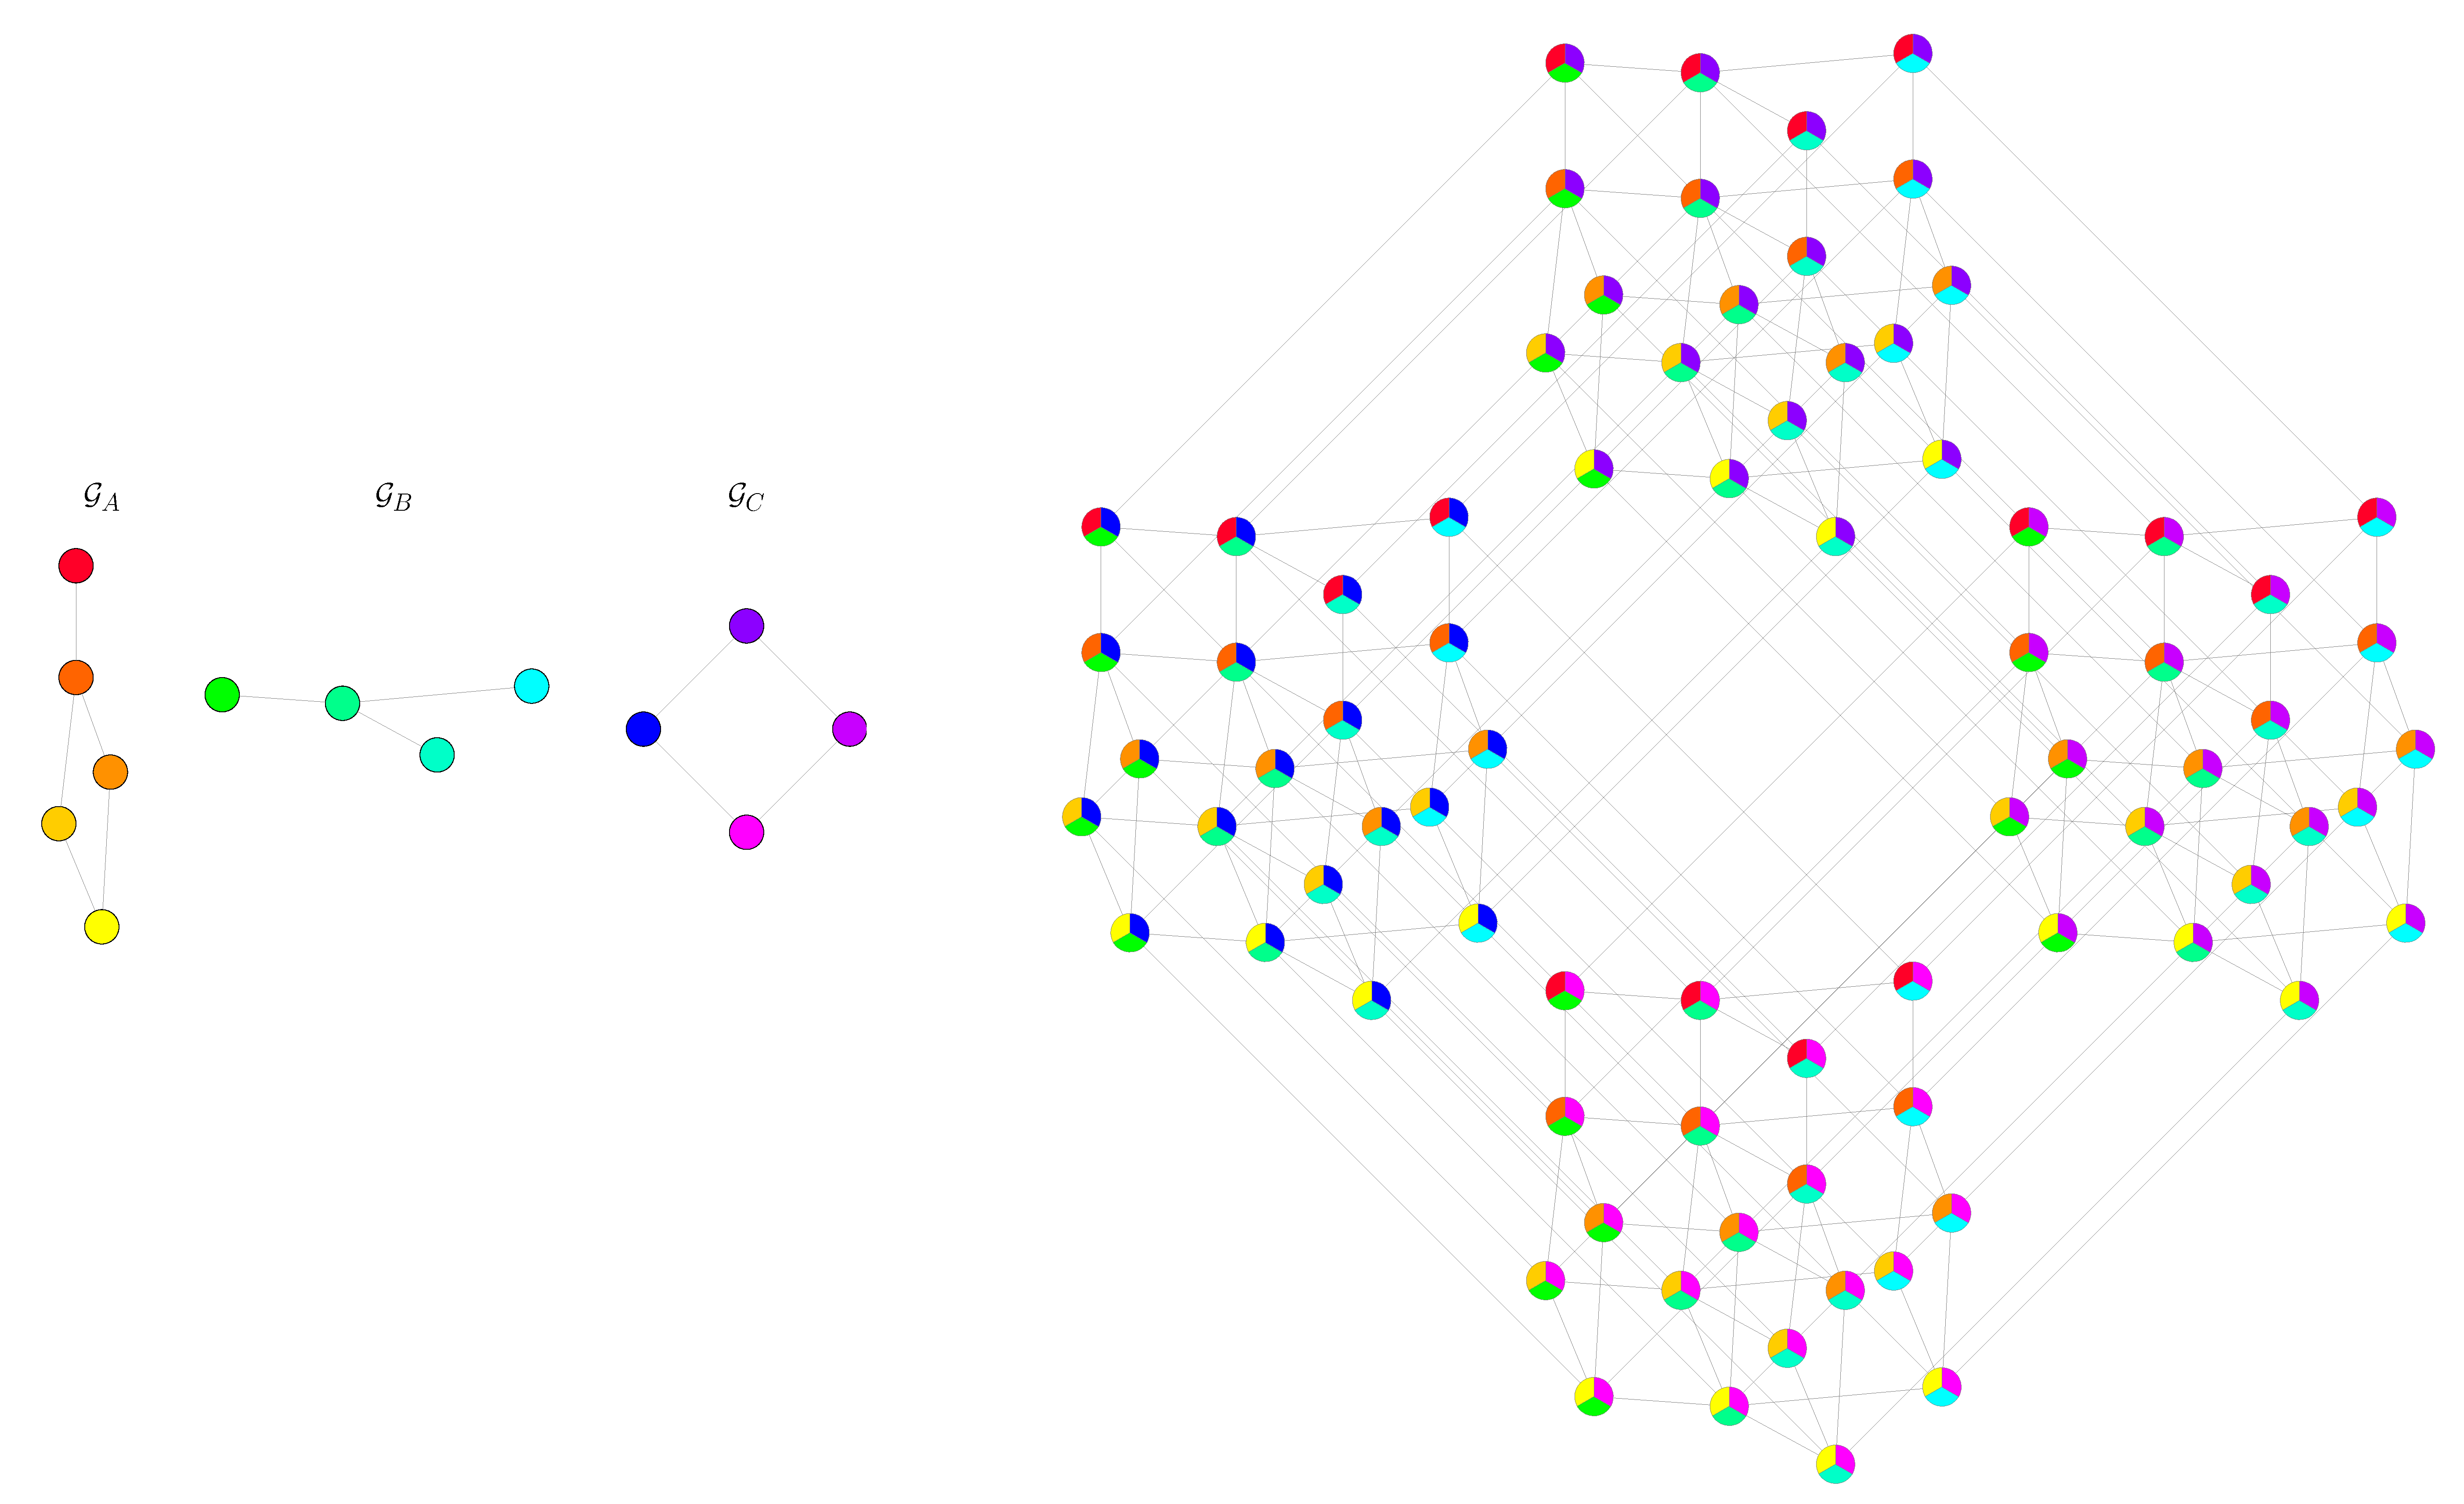
\includegraphics[width=\linewidth]{Figures/3D_CPG.pdf}
    \end{center}
    \caption[Graphical depiction of a 3D Cartesian product graph]{Graphical depiction of a 3D Cartesian product graph}
    \label{fig:3D_CPG}
\end{figure}

\Cref{fig:3D_CPG} gives a visual representation of a Cartesian product graph formed from three simple factor graphs. Notice that the size of the new vertex and edge set both grow very quickly. In particular, 

$$
|\mathcal{V}| = |\mathcal{V}_A| |\mathcal{V}_B| |\mathcal{V}_C| \aand |\mathcal{E}| =  |\mathcal{E}_A| |\mathcal{V}_B| |\mathcal{V}_C| + |\mathcal{V}_A| |\mathcal{E}_B| |\mathcal{V}_C| + |\mathcal{V}_A| |\mathcal{V}_B| |\mathcal{E}_C|
$$

Happily, the adjacency matrix of a Cartesian product graph $\A$ has a straightforward representation in terms of the factor adjacency matrices (here $\A_A$, $\A_B$ and $\A_C$). Specifically, it is given by the Kronecker sum

\begin{align}
    \A &= \A_A \oplus \A_B \oplus \A_C \notag \\
    &= \A_A \otimes \I_B \otimes \I_C  + \I_A \otimes \A_B \otimes \I_C + \I_A \otimes \I_B \otimes \A_C
\end{align}

In general, we can consider the Cartesian product of $d$ factor graphs with adjacency matrices denoted as $\A^{(1)} \in \R^{N_1 \times N_2}, \A^{(2)} \in \R^{N_2 \times N_2}, \dots \A^{(d)} \in \R^{N_d \times N_d}$. The full adjacency matrix will have size $N \times N$, where $N = \prod N_i$, and is given by  

\begin{alignat}{4}
    \A = \A^{(1)} & \oplus \A^{(2)} & \oplus \;\; ... \;\; & \oplus \A^{(d)} \notag \\[0.1cm]
    = \A^{(1)} & \otimes \I_{N_2} & \otimes \;\; ... \;\; & \otimes \I_{N_d} +  \notag \\[0.1cm]
    \I_{N_1} & \otimes \A^{(2)} & \otimes \;\; ... \;\; & \otimes \I_{N_d} + \;\; \ldots \;\; +  \notag \\[0.1cm]
    \I_{N_1} & \otimes \I_{N_2} & \otimes \;\; ... \;\; & \otimes \A^{(d)}  
\end{alignat}
    
This can be written compactly as 

\begin{equation}
    \A = \bigoplus_{i=1}^d  \A^{(i)}
\end{equation}

Similarly, the Laplacian of the product graph, $\LL$, can be written as the Kronecker sum of the individual factor graph Laplacians $\LL^{(i)}$. 

\begin{equation}
    \LL = \bigoplus_{i=1}^d  \LL^{(i)}
\end{equation}

We can perform eigendecomposition on each of the individual graph Laplacians as follows. 

\begin{equation}
    \LL^{(i)} = \U^{\,(i)} \LAM^{(i)} (\U^{\,(i)})^\top
\end{equation}

\noindent where $ \U^{(i)}$ is an orthogonal matrix such that each column is an eigenvector of $\LL^{(i)}$, and $\LAM^{(i)}$ is a diagonal matrix containing the corresponding eigenvalues, which are typically listed in ascending order. 

$$
\LAM^{(i)} = 
\begin{bmatrix}
    \lambda_1^{(i)}, &                 &        &                 \\
                     & \lambda_2^{(i)} &        &                 \\
                     &                 & \ddots &                 \\
                     &                 &        & \lambda_{N_i}^{(i)} \\
\end{bmatrix}
$$

Given this, the Laplacian of the product graph can be decomposed as follows. 

\begin{align}
    \LL &= \bigoplus_{i=1}^d \U^{\,(i)} \LAM^{(i)} (\U^{\,(i)})^\top \notag \\[0.2cm]
    &= \left( \bigotimes_{i=1}^d  \U^{\,(i)} \right) \left(\bigoplus_{i=1}^d \LAM^{(i)} \right) \left(\bigotimes_{i=1}^d  \U^{\,(i)} \right)^\top \notag \\[0.2cm]
    &= \U \LAM \U^\top 
\end{align}

\noindent where 

$$
\U =  \bigotimes_{i=1}^d  \U^{\,(i)} , \quad \text{and} \quad \LAM =  \bigoplus_{i=1}^d \LAM^{(i)}
$$

Here, we have used the notation $\bigotimes_{i=1}^d  \U^{\,(i)}$ to denote the chained Kronecker product of matrices $\{\U^{\,(i)}  \}$. 

\note{Tensor signals: notation and vectorisaion} {

A signal $\y$ residing on the nodes of a $d$-dimensional product graph has a natural representation as a rank-$d$ tensor which, for our purposes, can be conceptualised as a multi-dimensional array with $d$ independent axes. If the $i$-th factor graph has $N_i$ vertices, then $\y$ will be of shape $(N_1 \times N_2 \times ... \times N_d)$. An individual element of this tensor graph signal can be specified via a vector index $\mathbf{n} = [n_1,\, n_2,\, ...,\, n_d]$, where $1\leq n_i \leq N_i$. 

\vspace{0.5cm}

In the following, a tensor should be considered an element of a vector space, whereas square matrices such as $\LL, \U$ and $\LAM$, of shape $(N \times N)$ where $N = \prod N_i$, should be considered operators. These operators provide a linear map $\R^{N} \rightarrow \R^{N}$. For an operator to act on a graph signal we need a consistent way to map tensors of shape $(N_1 \times N_2 \times ... \times N_d)$ to vectors of length $N$. We refer to this process as \textit{vectorisation}. In order for the vectorisation process to be consistent with the operators, it should result in a vectors whose elements are arranged in \textit{lexicographic order}. A diagram showing the desired vectorisation operation for a rank-3 tensor is given below. 

\vspace{0.5cm}

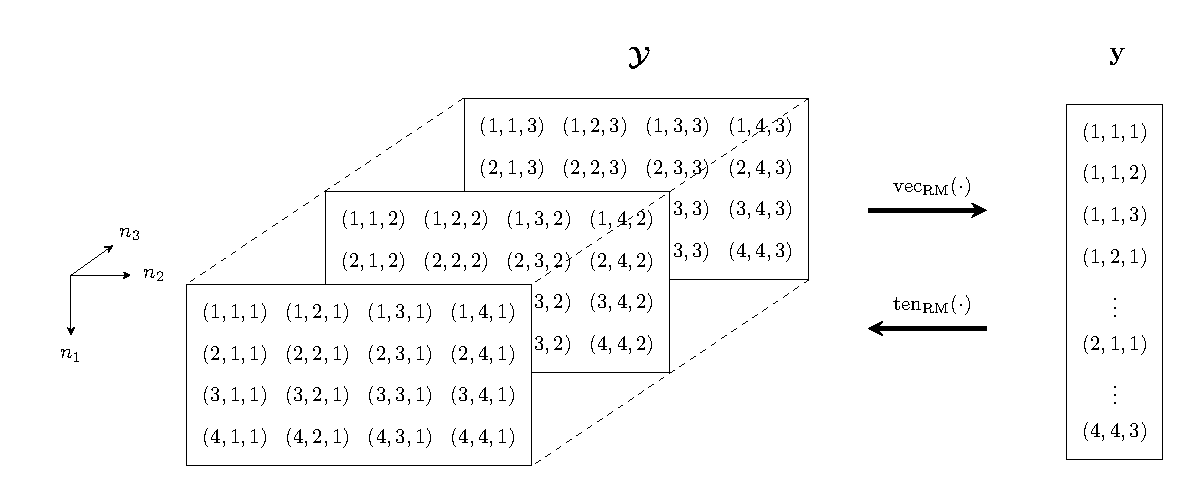
\includegraphics[width=\linewidth]{Figures/Tensor_Digaram.pdf}

\vspace{0.5cm}

This vectorisation process is sometimes referred to as \textit{row-major} since, in the 2D case, the index representing the row varies before the column index. Note that this is the default in languages such as C and Python's NumPy library \citep{harris2020}, but not in languages such as Fortran and Matlab in which the memory layout is instead organised in \textit{column-major} order. 

\vspace{0.5cm}

To calculate the vector element index $k$ which a tensor element with index $\mathbf{n} = [n_1,\, n_2,\, ...,\, n_d]$ is mapped to in row-major order, we can apply the following formula.  

\begin{equation}
    \label{eq:vec}
    k = 1 + \sum_{i=1}^d \Big( \prod_{j=i+1}^d N_i \Big) \, (n_i - 1)
\end{equation}

The reverse operation, i.e. mapping a vector element index $k$ to a tensor index $\mathbf{n}$ can be achieved by running the algorithm given below, 

\vspace{0.5cm}

\hrule

\vspace{0.2cm}

\begin{algorithmic}
\vspace{0.15cm}
\Require{The target vector element index $k$} 
\vspace{0.1cm}
\Require{The shape of the output tensor $(N_1, N_2, ..., N_d)$} 
\vspace{0.25cm}
\For{$i$ \textbf{from} $d$ \textbf{to} 1}
\vspace{0.25cm}
\State{$n_i \leftarrow  k \mod N_i$}
\vspace{0.15cm}
\State{$k \leftarrow \lfloor k / N_i \rfloor$} 
\vspace{0.15cm}
\EndFor
\vspace{0.25cm}
\Ensure{$(n_1 + 1, n_2 + 1, ..., n_d + 1)$}
\end{algorithmic}

\vspace{0.2cm}
\hrule

\vspace{0.5cm}

Given these two operations, two arrays of any consistent shape can be mapped between one another by first vectorising according to \cref{eq:vec}, and then converting to a tensor using the given algorithm.

}

A graph signal $\y$ existing on the nodes of a $d$-dimensional product graph can be represented as either a $d$-dimensional array (tensor) of shape $(N_1 \times N_2 \times ... \times N_d)$, or a vector of length $N = \prod_{i=1}^d N_i$. In the next section we discuss these two representations and how to convert between them in practice. For now, assume the signal is a length-$N$ vector. We can define its Graph Fourier Transform (GFT) and the corresponding inverse (IGFT) as follows. 

\begin{alignat}{2}
\label{eq:gft}
    \text{GFT}(\y) & = \U^\top \y && = \Big(  \bigotimes_{i=1}^d  \U^{\,(i)} \Big)^\top \y \\
\label{eq:igft}
    \text{IGFT}(\y) & = \U \y && = \Big(  \bigotimes_{i=1}^d  \U^{\,(i)} \Big) \; \y 
\end{alignat}

The concept of a graph filter for signals defined on a Cartesian product graph follows naturally from this definition. In particular, in the simplest case, we can consider an isotropic graph filter function, such as one of those defined in \cref{tab:iso_filters}, applied to the product graph Laplacian. 

\begin{align}
    \HH &= g\left(\bigoplus_{i=1}^d  \LL^{(i)}; \beta\right) \notag \\[0.2cm]
        &= \left( \bigotimes_{i=1}^d  \U^{\,(i)} \right) g\left(\bigoplus_{i=1}^d \LAM^{(i)}; \beta \right) \left(\bigotimes_{i=1}^d  \U^{\,(i)} \right)^\top \notag \\[0.2cm]
        &= \U \, \Diag{\vecrm{\G}} \, \U^\top
\end{align}

where $\G$ now represents the spectral scaling \textit{tensor}, which has elements given by 

\begin{equation}
    \G_{\mathbf{n}} = g\left(\sum_{i=1}^d \lambda^{i}_{n_i}; \, \beta\right)
\end{equation}

This can be further generalised to a anisotropic graph filter function, where the intensity of the filtering operation is not restricted to be equal in each dimension. In this case, the spectral scaling tensor is given by 

\begin{equation}
    \G_{\mathbf{n}} = g(\lambdaa_{\mathbf{n}}; \betaa)
\end{equation}

where 

$$
\mathbf{n} = \begin{bmatrix}
    n_1 \\ n_2 \\ \vdots \\ n_d
\end{bmatrix}
\aand \lambdaa_{\mathbf{n}} = 
\begin{bmatrix}
    \lambda^{(1)}_{n_1} \\ \lambda^{(2)}_{n_2} \\ \vdots \\ \lambda^{(d)}_{n_d}    
\end{bmatrix}
$$

\section{Fast computation with \textit{d}-dimensional Kronecker products}

Hello

\section{Signal reconstruction}

Hello

\section{Kernel Graph Regression}

Hello

\section{Regression with Network Cohesion}

Ahhhh

\section{Regression with Network Cohesion}